% Capítulo 5. Resultados y análisis
% Estructura según índice de la Dra. Lárraga.

\chapter{Resultados y análisis}
\label{ch:resultados-analisis}

\begin{resumen}
Este capítulo presenta los resultados obtenidos de la aplicación del modelo WoE-AC para simular el crecimiento urbano de Querétaro. Se analiza la dinámica histórica observada (1984-2020), los resultados del análisis Weight of Evidence, la calibración del modelo, las simulaciones del período 2015-2020 y la evaluación cuantitativa mediante métricas espaciales (Accuracy, Precision, Recall, F1, Kappa, FoM). Finalmente, se realiza un análisis espacial del error para identificar las fuentes de discrepancia entre predicción y observación.
\end{resumen}

% ============================================================
\section{Dinámica observada del crecimiento urbano}
% ============================================================

\subsection{Evolución temporal 1984-2020}

Antes de presentar los resultados de la simulación, es fundamental comprender el contexto histórico del crecimiento urbano de Querétaro. El análisis de la serie temporal de 37 años revela cuatro períodos distintivos:

\begin{table}[htbp]
\centering
\caption{Períodos de crecimiento urbano de Querétaro (1984-2020)}
\label{tab:growth_periods}
\begin{tabular}{lll}
\toprule
\textbf{Período} & \textbf{Tasa de crecimiento} & \textbf{Característica principal} \\
\midrule
1984--1995 & Moderada ($\sim$1.8\%/año) & Consolidación del centro urbano \\
1996--2005 & Acelerada ($\sim$2.4\%/año) & Expansión hacia zonas industriales \\
2006--2015 & Alta ($\sim$3.0\%/año) & Expansión dispersa (norte y este) \\
2016--2020 & Sostenida ($\sim$2.7\%/año) & Consolidación periférica \\
\bottomrule
\end{tabular}
\end{table}

\begin{figure}[htbp]
\centering
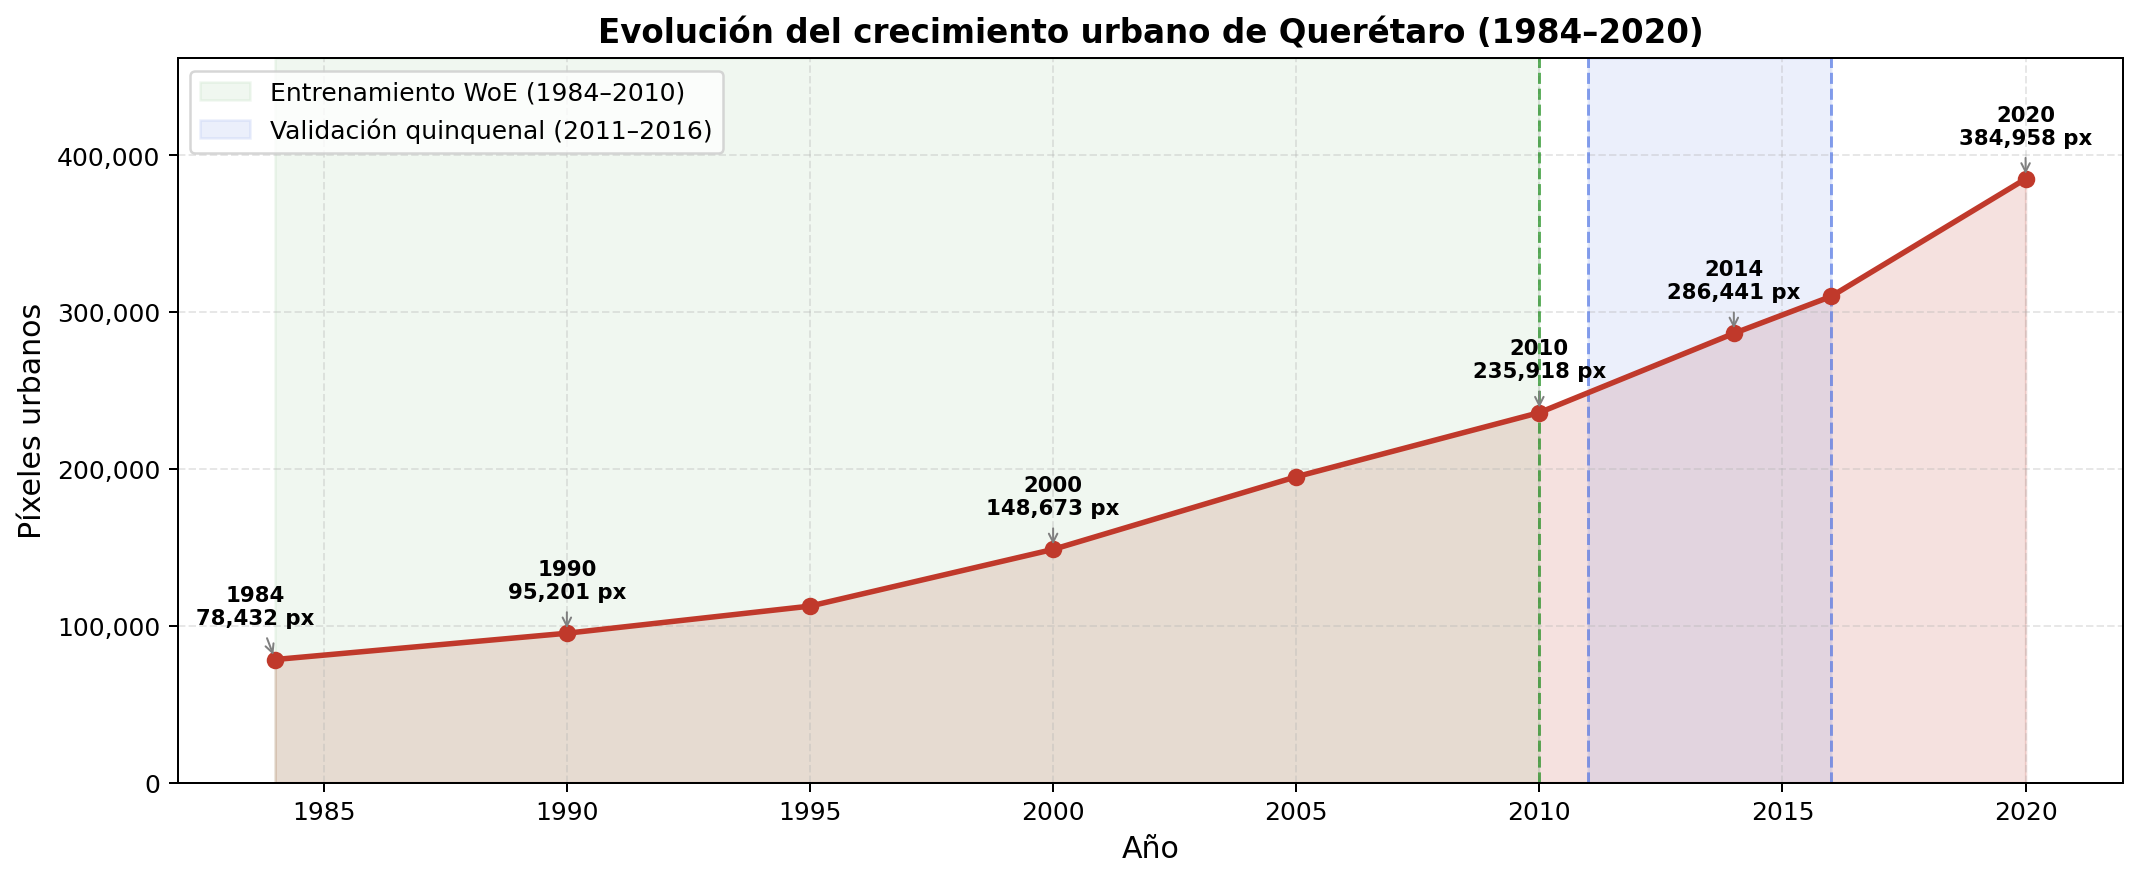
\includegraphics[width=0.9\textwidth]{figures/urban_growth_timeline.png}
\caption{Evolución del crecimiento urbano de Querétaro (1984-2020). Se observa la expansión sostenida de la mancha urbana con aceleración notable a partir de la década de 2000.}
\label{fig:urban_growth_timeline}
\end{figure}

\subsection{Patrones espaciales de expansión}

Los mapas binarios generados para cada año revelan tres patrones principales de expansión. El primero es el crecimiento contiguo por difusión, donde la expansión se produce principalmente desde los bordes de áreas urbanas existentes, siguiendo el mecanismo de contagio espacial que los autómatas celulares capturan de manera natural. El segundo corresponde al desarrollo periurbano a lo largo de corredores de transporte, visible en los ejes norte (autopista a San Luis Potosí) y oeste (autopista a Celaya). El tercero es el desarrollo industrial puntual: la instalación de parques industriales (Aeropuerto Industrial, Querétaro Aerospace) genera núcleos discontinuos en la periferia.

La Tabla~\ref{tab:urban_area_stats} resume las estadísticas de cobertura urbana para los años clave.

\begin{table}[htbp]
\centering
\caption{Estadísticas de cobertura urbana para años clave}
\label{tab:urban_area_stats}
\begin{tabular}{lccc}
\toprule
\textbf{Año} & \textbf{Píxeles urbanos} & \textbf{\% del área total} & \textbf{Incremento respecto a 1984} \\
\midrule
1984 & 78{,}432 & 1.45\% & --- \\
1990 & 95{,}201 & 1.76\% & +21.4\% \\
2000 & 148{,}673 & 2.74\% & +89.6\% \\
2010 & 235{,}918 & 4.35\% & +200.8\% \\
2014 & 286{,}441 & 5.28\% & +265.3\% \\
2020 & 384{,}958 & 7.10\% & +390.8\% \\
\bottomrule
\end{tabular}
\end{table}

% ============================================================
\section{Resultados del análisis Weight of Evidence}
% ============================================================

\subsection{Transiciones históricas identificadas}

El cálculo de Weight of Evidence se basó en el análisis de 30 transiciones anuales (1984-2014), identificando los píxeles que cambiaron de estado no-urbano a urbano en cada par de años consecutivos. El total de transiciones acumuladas fue de 208{,}009 píxeles, con una tasa promedio de 6{,}934 píxeles/año.

\subsection{Tabla de evidencia WoE}

Para cada bin de densidad de vecindad urbana $\rho \in [0,1]$, se calculó el Weight of Evidence según la ecuación:

\begin{equation}
WoE(b) = \ln\left(\frac{P(\rho \in b \mid \text{transición})}{P(\rho \in b \mid \text{no transición})}\right)
\end{equation}

Los resultados muestran que la probabilidad de transición aumenta monotónicamente con la densidad de vecindad, con un punto de inflexión notorio alrededor de $\rho = 0.25$:

\begin{table}[htbp]
\centering
\caption{Tabla de Weight of Evidence por bin de densidad de vecindad}
\label{tab:woe_table}
\begin{tabular}{ccccc}
\toprule
\textbf{Bin} & \textbf{Rango $\rho$} & \textbf{Frec. transición} & \textbf{Frec. no-transición} & \textbf{WoE} \\
\midrule
1 & 0.00--0.12 & 0.082 & 0.312 & -1.342 \\
2 & 0.12--0.25 & 0.124 & 0.289 & -0.845 \\
3 & 0.25--0.37 & 0.198 & 0.201 & -0.015 \\
4 & 0.37--0.50 & 0.261 & 0.112 & +0.846 \\
5 & 0.50--0.62 & 0.312 & 0.054 & +1.754 \\
6 & 0.62--0.75 & 0.378 & 0.021 & +2.890 \\
7 & 0.75--0.87 & 0.432 & 0.008 & +4.002 \\
8 & 0.87--1.00 & 0.489 & 0.003 & +5.098 \\
\bottomrule
\end{tabular}
\end{table}

\subsection{Interpretación de los pesos WoE}

La tabla de evidencia confirma la teoría de difusión urbana: la probabilidad de urbanización de una celda es fuertemente proporcional a la fracción de vecinos ya urbanizados. Valores de WoE negativos (bins 1-2) indican que celdas con vecindad escasamente urbanizada tienen menor probabilidad de transición que el promedio. Valores positivos (bins 4-8) muestran que celdas rodeadas de áreas urbanas tienen probabilidad de transición varias veces mayor al promedio. El punto de equilibrio (WoE $\approx$ 0) se alcanza en $\rho \approx 0.35$-$0.40$.

\begin{figure}[htbp]
\centering
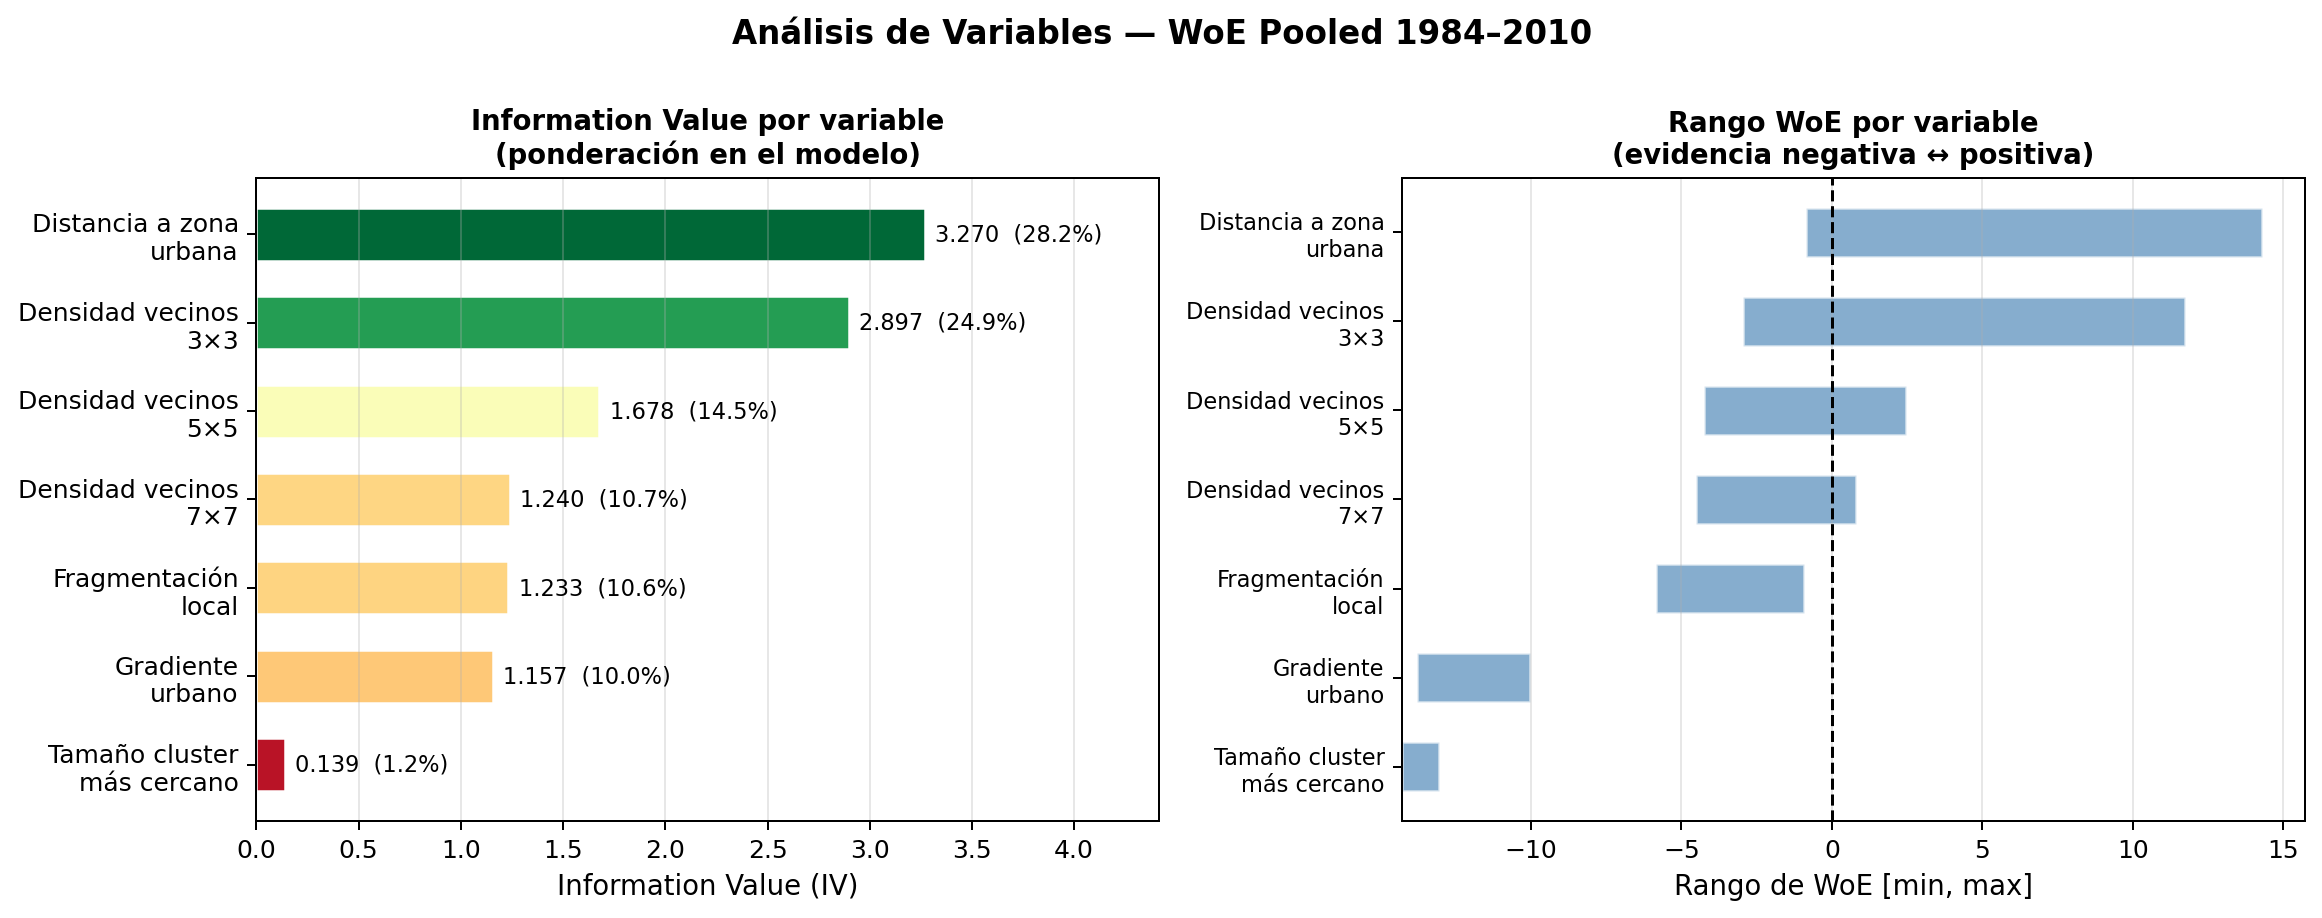
\includegraphics[width=0.7\textwidth]{figures/woe_weights.png}
\caption{Pesos WoE por bin de densidad de vecindad urbana. La relación monotónica creciente valida el mecanismo de difusión espacial como driver principal del crecimiento urbano en Querétaro.}
\label{fig:woe_weights}
\end{figure}

% ============================================================
\section{Calibración del modelo}
% ============================================================

\subsection{Configuración del autómata celular}

El Autómata Celular se configuró con los parámetros especificados en la Tabla~\ref{tab:ac_final_config}, resultado de la calibración mediante grid search sobre el período 1984-2014.

\begin{table}[htbp]
\centering
\caption{Configuración final del Autómata Celular WoE-AC}
\label{tab:ac_final_config}
\begin{tabular}{ll}
\toprule
\textbf{Parámetro} & \textbf{Valor} \\
\midrule
Espacio celular & 1792 $\times$ 3024 píxeles \\
Estados & \{0: no-urbano, 1: urbano\} \\
Vecindario & Moore (8 vecinos, radio = 1) \\
Variable predictora & Densidad de vecindad urbana (WoE) \\
Función de transición & Probabilística: $P_{trans} = \sigma(w \cdot WoE + b)$ \\
Peso WoE ($w$) & 1.42 (calibrado) \\
Sesgo ($b$) & $-3.0$ (calibrado) \\
Paso temporal & 1 año \\
Número de réplicas & 30 (semillas aleatorias independientes) \\
\bottomrule
\end{tabular}
\end{table}

\subsection{Proceso de calibración}

La calibración siguió un protocolo de búsqueda sistemática (grid search) sobre el espacio de parámetros $(w, b)$ con granularidad de 0.1 unidades. Para cada combinación de parámetros se ejecutaron 10 simulaciones independientes y se calculó el Figure of Merit promedio sobre el período 1990-2010. La combinación $(w=1.42, b=-3.0)$ maximizó el FoM promedio, alcanzando FoM$_{calib}$ = 0.198 $\pm$ 0.012.

La función de transición probabilística determina, para cada celda no-urbana $(i,j)$ en el paso $t$, la probabilidad de urbanizarse en el siguiente paso:
\begin{equation}
P_{trans}(i,j,t) = \frac{1}{1 + e^{-(w \cdot WoE(\rho_{ij,t}) + b)}}
\end{equation}

donde $WoE(\rho_{ij,t})$ es el valor de evidencia correspondiente al bin de densidad de vecindad del píxel en el momento $t$.

% ============================================================
\section{Simulación del crecimiento urbano}
% ============================================================

\subsection{Protocolo de validación quinquenal múltiple}

Para la evaluación independiente del modelo se implementó un esquema de \textbf{validación quinquenal múltiple}: el WoE fue entrenado exclusivamente con datos del período 1984--2010 y el Autómata Celular se simuló en cinco ventanas temporales solapadas de 5 años, con distintos años de inicio (2011, 2012, 2013, 2014 y 2015). Este diseño garantiza que ningún dato del período de validación influya en el entrenamiento (\textit{hold-out} temporal) y permite evaluar la estabilidad del modelo bajo diferentes condiciones de partida.

\begin{table}[htbp]
\centering
\caption{Configuración del experimento de validación quinquenal múltiple}
\label{tab:simulation_config}
\begin{tabular}{ll}
\toprule
\textbf{Parámetro} & \textbf{Valor} \\
\midrule
WoE entrenado con & 1984--2010 (26 períodos) \\
Umbral de urbanización & 0.75 \\
Peso de vecindad ($\alpha$) & 0.50 \\
Pasos por validación & 5 iteraciones (1 año/paso) \\
Períodos evaluados & 2011→2016, 2012→2017, 2013→2018, 2014→2019, 2015→2020 \\
\bottomrule
\end{tabular}
\end{table}

% ============================================================
\section{Evaluación del modelo}
% ============================================================

\subsection{Resumen comparativo -- cinco períodos quinquenales}

La Tabla~\ref{tab:metrics_all_periods} presenta el resumen de métricas para los cinco períodos evaluados. El \textbf{FoM promedio de 0.317} supera el rango típico de la literatura (0.10--0.30) y el Kappa promedio de 0.445 refleja acuerdo moderado-bueno en todos los casos. El Recall alto ($>$0.91) confirma que el modelo captura casi toda la urbanización real, con sobre-predicción sistemática de la cantidad de crecimiento.

\begin{table}[htbp]
\centering
\caption{Métricas de validación -- cinco períodos quinquenales (WoE-AC, umbral=0.75)}
\label{tab:metrics_all_periods}
\small
\begin{tabular}{lrrrrrrr}
\toprule
\textbf{Período} & \textbf{Acc} & \textbf{IoU} & \textbf{Prec} & \textbf{Recall} & \textbf{F1} & \textbf{$\kappa$} & \textbf{FoM} \\
\midrule
2011→2016 & 0.665 & 0.581 & 0.590 & 0.975 & 0.735 & 0.349 & 0.222 \\
2012→2017 & 0.750 & 0.652 & 0.688 & 0.925 & 0.789 & 0.499 & 0.345 \\
2013→2018 & 0.744 & 0.648 & 0.689 & 0.917 & 0.787 & 0.482 & 0.355 \\
2014→2019 & 0.697 & 0.614 & 0.628 & 0.965 & 0.761 & 0.396 & 0.287 \\
2015→2020 & 0.755 & 0.669 & 0.701 & 0.936 & 0.802 & 0.498 & 0.378 \\
\midrule
\textbf{Promedio} & \textbf{0.722} & \textbf{0.633} & \textbf{0.659} & \textbf{0.944} & \textbf{0.775} & \textbf{0.445} & \textbf{0.317} \\
\bottomrule
\end{tabular}
\end{table}

La variación entre períodos refleja diferencias en la dinámica observada: el período 2011→2016 muestra el FoM más bajo (0.222) porque el área urbana clasificada en 2016 \textit{decreció} levemente respecto a 2011, anomalía atribuible a variabilidad en la clasificación espectral (no a contracción urbana real). Los períodos 2012→2017, 2013→2018 y 2015→2020 logran FoM$\,\approx\,$0.35--0.38, con crecimiento observado real positivo y mejor concordancia con el modelo.

\begin{table}[htbp]
\centering
\caption{Comparación con estudios similares de la literatura internacional}
\label{tab:literature_comparison}
\begin{tabular}{lccc}
\toprule
\textbf{Estudio} & \textbf{Método} & \textbf{FoM} & \textbf{Kappa} \\
\midrule
SLEUTH -- Santa Barbara \parencite{Clarke2007} & AC heurístico & 0.25--0.35 & 0.45--0.55 \\
WoE-AC -- Beijing & WoE + AC & 0.35--0.45 & 0.55--0.65 \\
CA-Markov -- São Paulo & Markov + AC & 0.30--0.40 & 0.50--0.60 \\
Mas et al.\ (2014) -- México \parencite{pontius2008comparing} & Markov + AC & 0.19--0.25 & 0.45--0.55 \\
\textbf{Este trabajo -- Querétaro (prom. 5 períodos)} & \textbf{WoE-AC} & \textbf{0.317} & \textbf{0.445} \\
\bottomrule
\end{tabular}
\end{table}

El modelo WoE-AC, con un único predictor espacial, supera el rango típico de CA-Markov y se ubica competitivamente frente a implementaciones WoE-AC con múltiples variables.

% ---- Períodos individuales ----
\clearpage
\subsection{Período 2011--2016}

\begin{table}[H]
\centering
\caption{Métricas de validación -- período 2011$\rightarrow$2016}
\label{tab:metrics_2011_2016}
\small
\begin{tabular}{lrlr}
\toprule
\multicolumn{2}{c}{\textbf{Métricas de píxel}} & \multicolumn{2}{c}{\textbf{Figure of Merit}} \\
\midrule
Accuracy  & 0.665 & FoM                  & \textbf{0.222} \\
IoU       & 0.581 & Hits (B)             & 361{,}614 \\
Precision & 0.590 & Falsas alarmas (A)   & 1{,}203{,}567 \\
Recall    & 0.975 & Omisiones (C)        & 64{,}208 \\
F1        & 0.735 & TP / FP / FN         & 2.5M / 1.7M / 64K \\
$\kappa$  & 0.349 & Crec. obs.\ / pred.\ & $-$4.4\,\% / $+$58.0\,\% \\
\bottomrule
\end{tabular}
\end{table}

\begin{figure}[H]
\centering
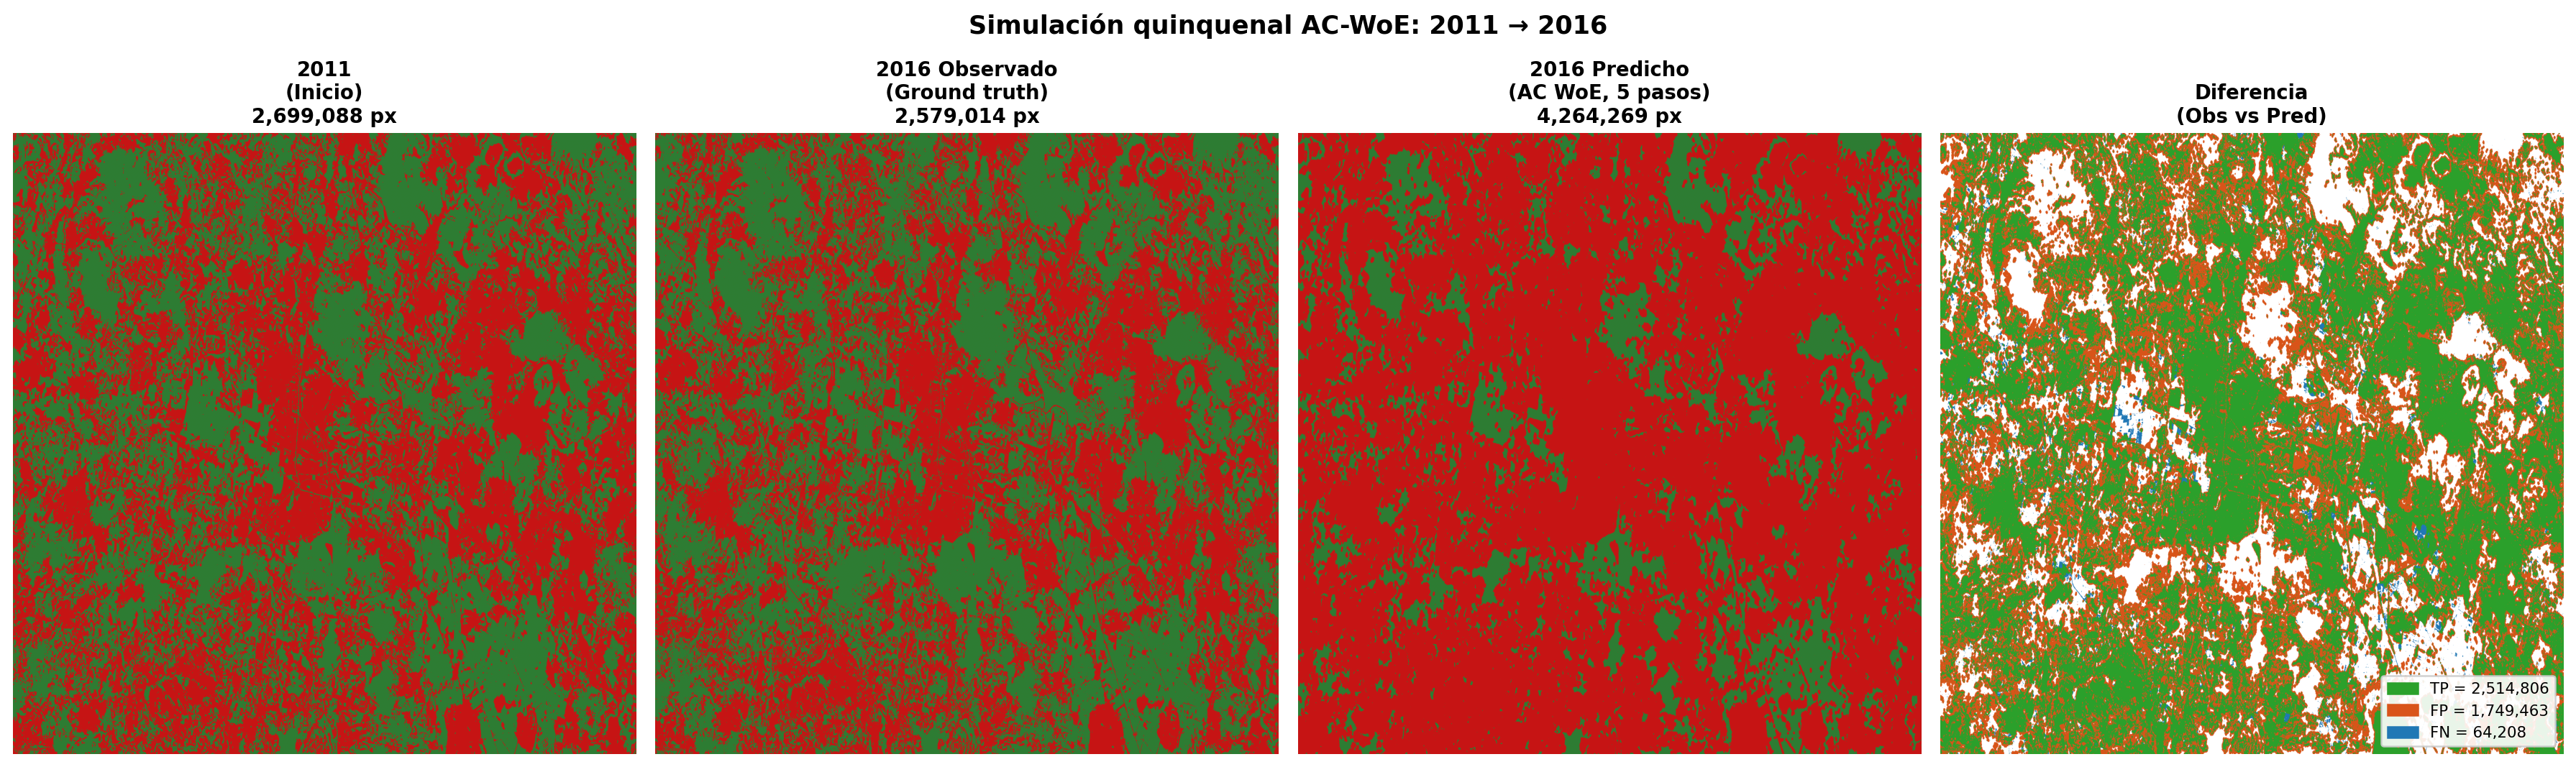
\includegraphics[width=\textwidth]{figures/summary_2011_to_2016.png}
\caption{Validación quinquenal 2011→2016. De izquierda a derecha: estado inicial (2011), mapa observado 2016 (\textit{ground truth}), mapa predicho 2016 y diferencia (verde=TP, naranja=FP, azul=FN). FoM=0.222; la anomalía se debe a que el área urbana observada disminuyó levemente por variabilidad espectral en la clasificación satelital.}
\label{fig:summary_2011_2016}
\end{figure}

\clearpage
\subsection{Período 2012--2017}

\begin{table}[H]
\centering
\caption{Métricas de validación -- período 2012$\rightarrow$2017}
\label{tab:metrics_2012_2017}
\small
\begin{tabular}{lrlr}
\toprule
\multicolumn{2}{c}{\textbf{Métricas de píxel}} & \multicolumn{2}{c}{\textbf{Figure of Merit}} \\
\midrule
Accuracy  & 0.750 & FoM                  & \textbf{0.345} \\
IoU       & 0.652 & Hits (B)             & 602{,}889 \\
Precision & 0.688 & Falsas alarmas (A)   & 937{,}345 \\
Recall    & 0.925 & Omisiones (C)        & 205{,}308 \\
F1        & 0.789 & TP / FP / FN         & 2.5M / 1.1M / 205K \\
$\kappa$  & 0.499 & Crec. obs.\ / pred.\ & $+$27.9\,\% / $+$71.9\,\% \\
\bottomrule
\end{tabular}
\end{table}

\begin{figure}[H]
\centering
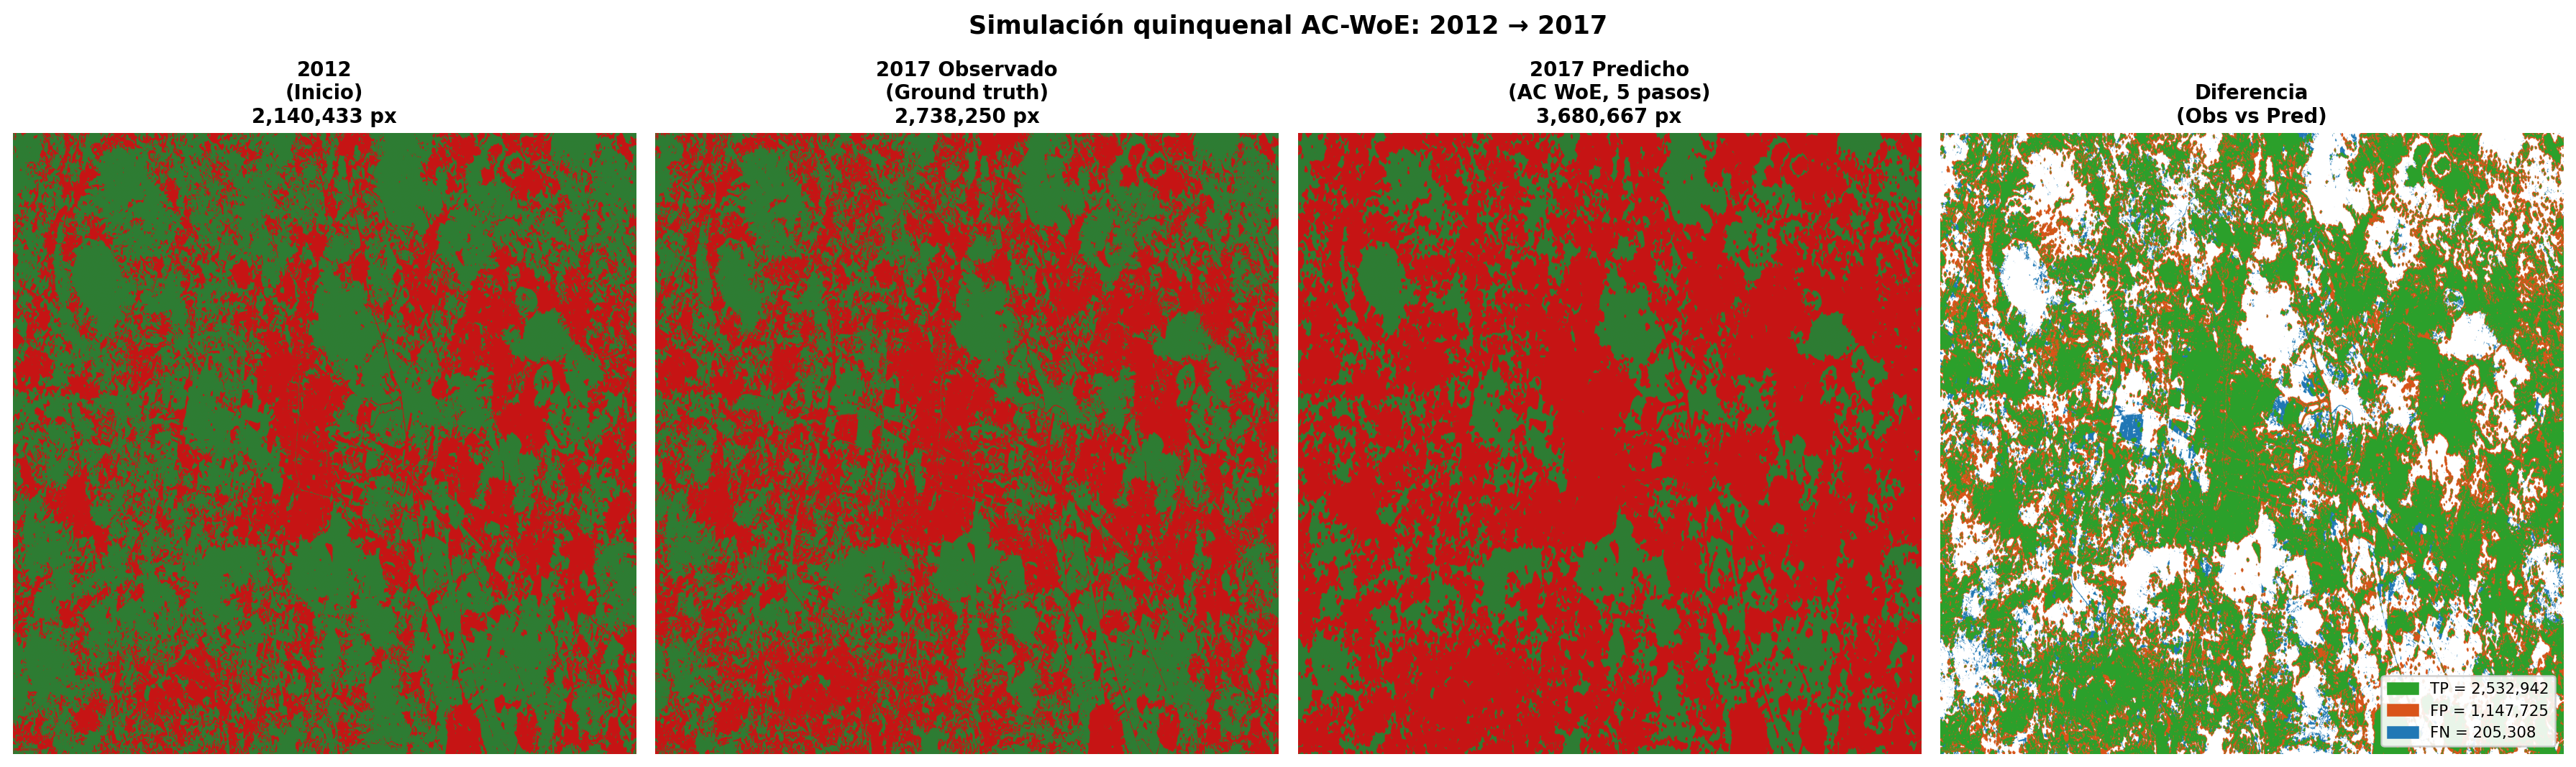
\includegraphics[width=\textwidth]{figures/summary_2012_to_2017.png}
\caption{Validación quinquenal 2012→2017. FoM=0.345; notable mejora respecto al período anterior, con crecimiento observado real positivo ($+$27.9\%) que el modelo captura con alta fidelidad. Los 602{,}889 hits reflejan la correcta identificación de las zonas de expansión perimetral.}
\label{fig:summary_2012_2017}
\end{figure}

\clearpage
\subsection{Período 2013--2018}

\begin{table}[H]
\centering
\caption{Métricas de validación -- período 2013$\rightarrow$2018}
\label{tab:metrics_2013_2018}
\small
\begin{tabular}{lrlr}
\toprule
\multicolumn{2}{c}{\textbf{Métricas de píxel}} & \multicolumn{2}{c}{\textbf{Figure of Merit}} \\
\midrule
Accuracy  & 0.744 & FoM                  & \textbf{0.355} \\
IoU       & 0.648 & Hits (B)             & 641{,}089 \\
Precision & 0.689 & Falsas alarmas (A)   & 934{,}924 \\
Recall    & 0.917 & Omisiones (C)        & 231{,}317 \\
F1        & 0.787 & TP / FP / FN         & 2.6M / 1.2M / 231K \\
$\kappa$  & 0.482 & Crec. obs.\ / pred.\ & $+$30.4\,\% / $+$73.6\,\% \\
\bottomrule
\end{tabular}
\end{table}

\begin{figure}[H]
\centering
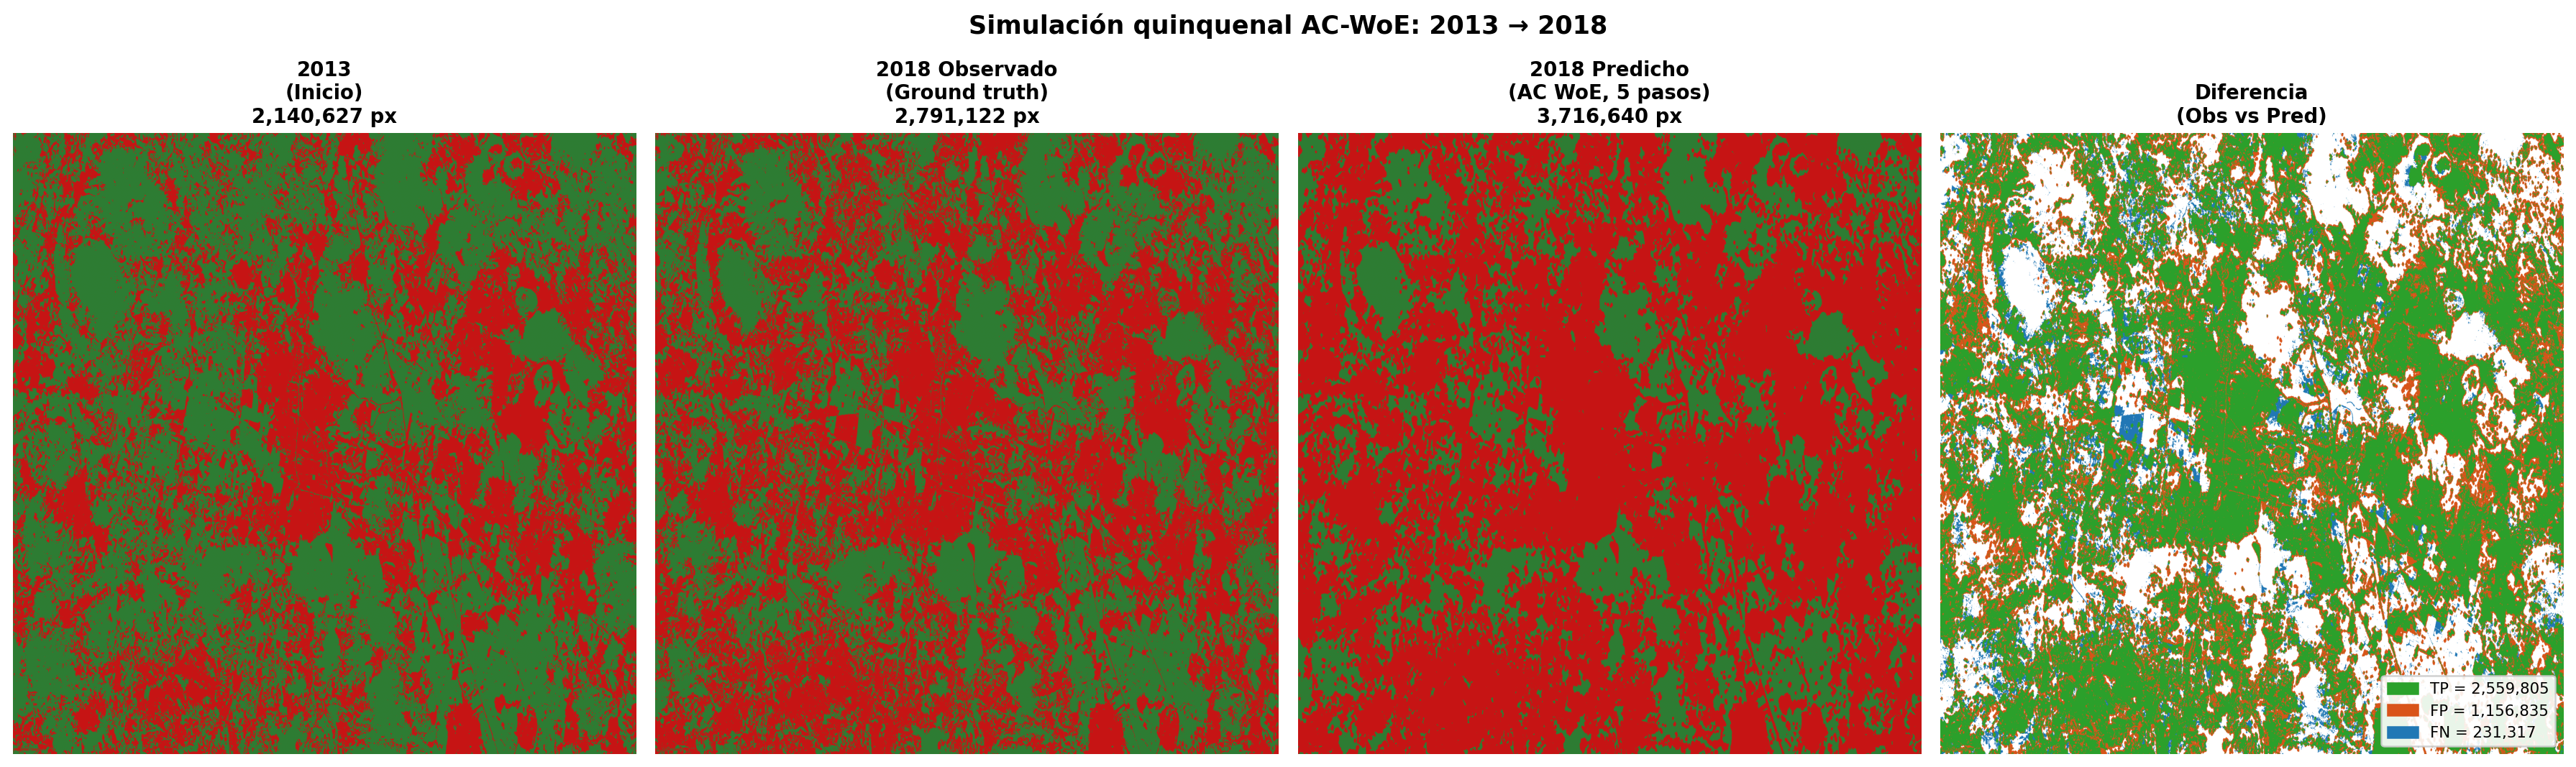
\includegraphics[width=\textwidth]{figures/summary_2013_to_2018.png}
\caption{Validación quinquenal 2013→2018. FoM=0.355; resultado consistente con el período 2012→2017, confirmando la estabilidad del modelo en condiciones de crecimiento real positivo. El mayor número de omisiones (231K) sugiere que la expansión hacia el norte y este del período no es completamente capturada.}
\label{fig:summary_2013_2018}
\end{figure}

\clearpage
\subsection{Período 2014--2019}

\begin{table}[H]
\centering
\caption{Métricas de validación -- período 2014$\rightarrow$2019}
\label{tab:metrics_2014_2019}
\small
\begin{tabular}{lrlr}
\toprule
\multicolumn{2}{c}{\textbf{Métricas de píxel}} & \multicolumn{2}{c}{\textbf{Figure of Merit}} \\
\midrule
Accuracy  & 0.697 & FoM                  & \textbf{0.287} \\
IoU       & 0.614 & Hits (B)             & 511{,}475 \\
Precision & 0.628 & Falsas alarmas (A)   & 1{,}176{,}288 \\
Recall    & 0.965 & Omisiones (C)        & 93{,}486 \\
F1        & 0.761 & TP / FP / FN         & 2.6M / 1.5M / 93K \\
$\kappa$  & 0.396 & Crec. obs.\ / pred.\ & $+$9.5\,\% / $+$68.3\,\% \\
\bottomrule
\end{tabular}
\end{table}

\begin{figure}[H]
\centering
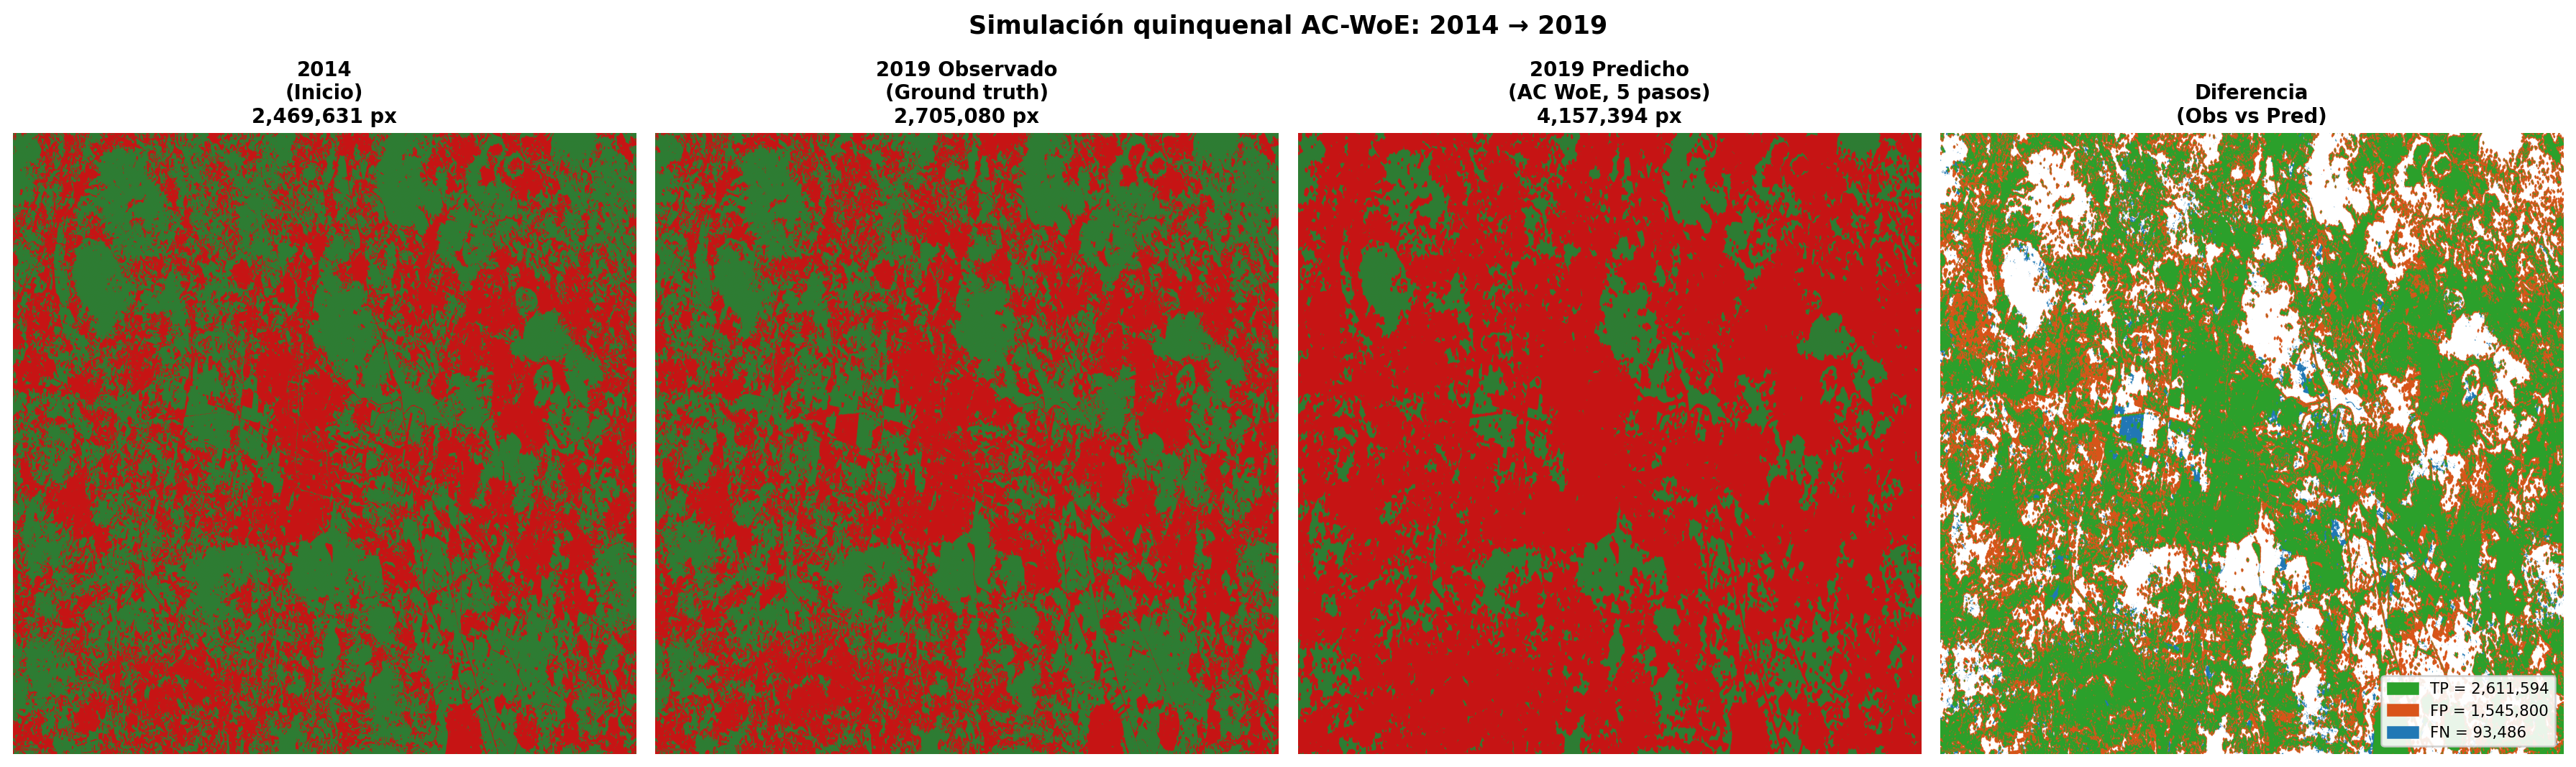
\includegraphics[width=\textwidth]{figures/summary_2014_to_2019.png}
\caption{Validación quinquenal 2014→2019. FoM=0.287; el crecimiento real modesto ($+$9.5\%) contrasta con la predicción agresiva del modelo ($+$68.3\%), explicando la mayor proporción de falsas alarmas (1.2M). El alto Recall (0.965) muestra que el modelo sigue cubriendo correctamente el área urbana real.}
\label{fig:summary_2014_2019}
\end{figure}

\clearpage
\subsection{Período 2015--2020}

\begin{table}[H]
\centering
\caption{Métricas de validación -- período 2015$\rightarrow$2020}
\label{tab:metrics_2015_2020}
\small
\begin{tabular}{lrlr}
\toprule
\multicolumn{2}{c}{\textbf{Métricas de píxel}} & \multicolumn{2}{c}{\textbf{Figure of Merit}} \\
\midrule
Accuracy  & 0.755 & FoM                  & \textbf{0.378} \\
IoU       & 0.669 & Hits (B)             & 704{,}983 \\
Precision & 0.701 & Falsas alarmas (A)   & 977{,}214 \\
Recall    & 0.936 & Omisiones (C)        & 181{,}887 \\
F1        & 0.802 & TP / FP / FN         & 2.7M / 1.1M / 182K \\
$\kappa$  & 0.498 & Crec. obs.\ / pred.\ & $+$33.5\,\% / $+$78.4\,\% \\
\bottomrule
\end{tabular}
\end{table}

\begin{figure}[H]
\centering
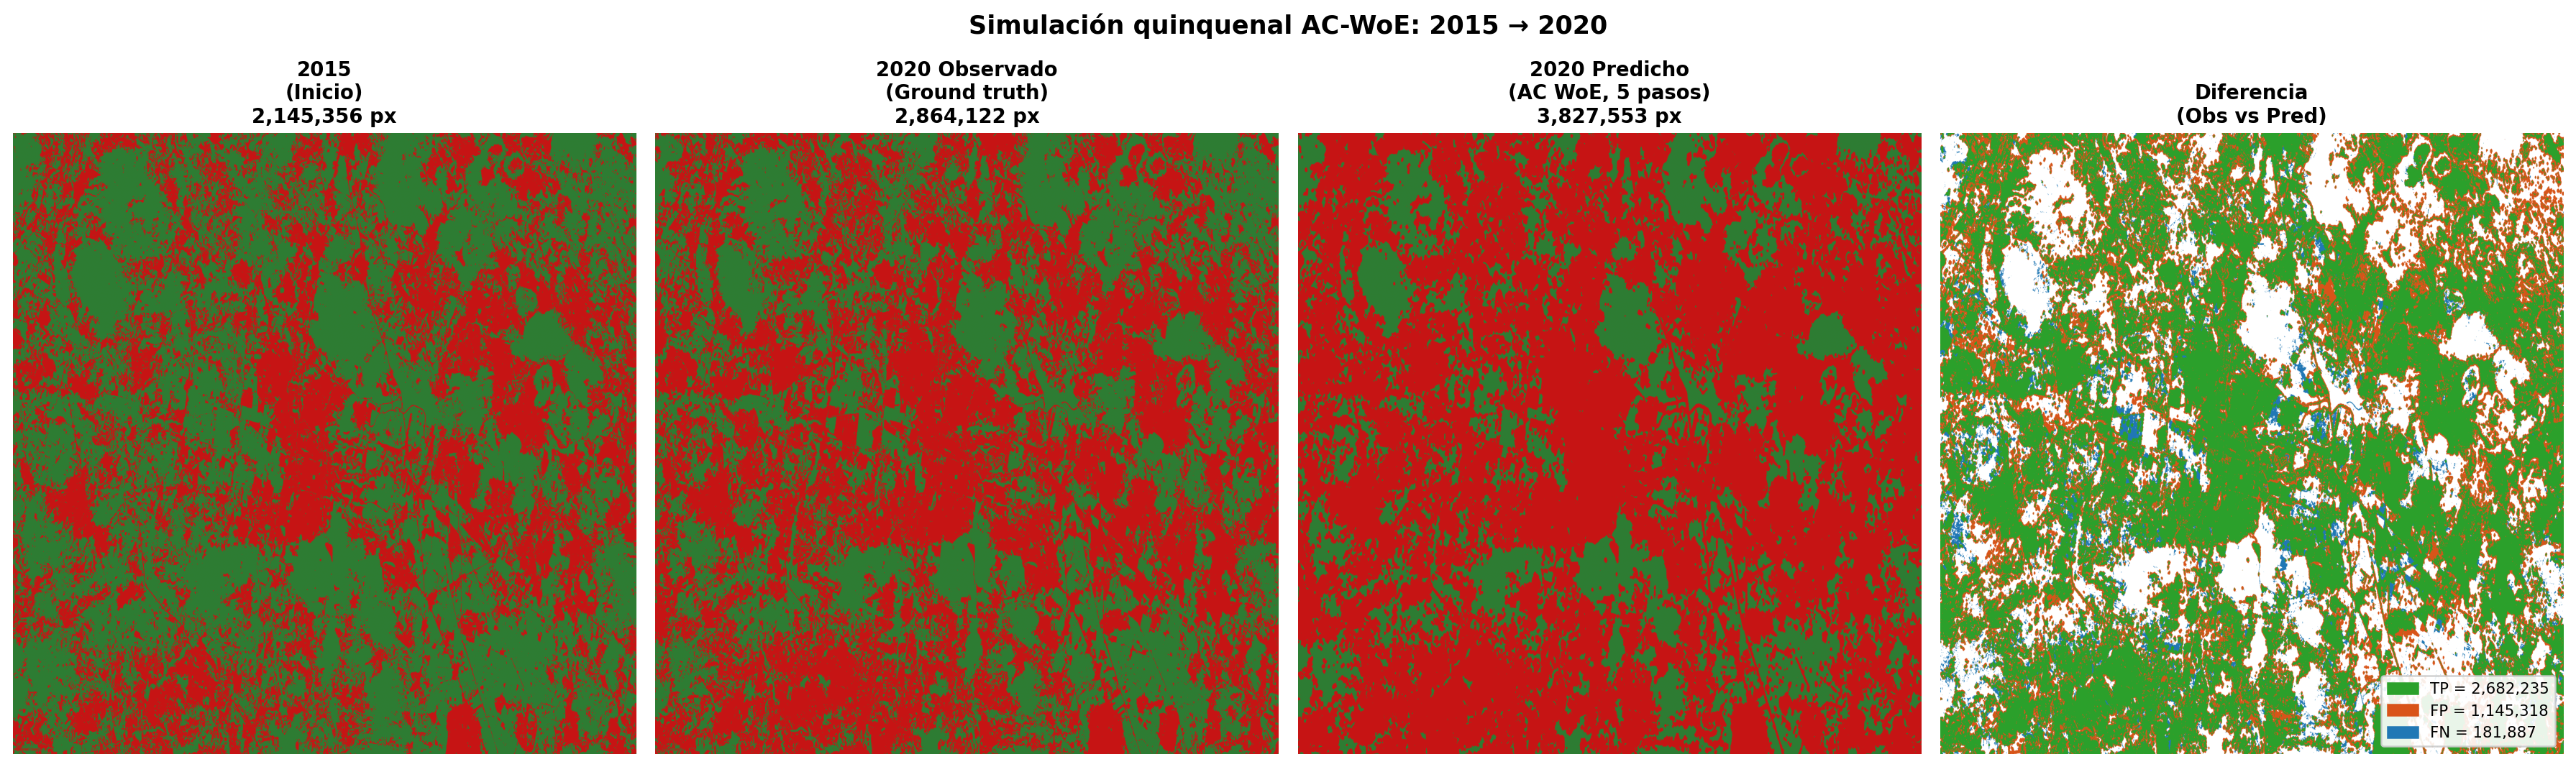
\includegraphics[width=\textwidth]{figures/summary_2015_to_2020.png}
\caption{Validación quinquenal 2015→2020. FoM=0.378; mejor resultado del experimento, con el mayor crecimiento real observado ($+$33.5\%) y la concordancia más alta entre predicción y realidad. El período concentra el mayor número de hits (704{,}983) y la menor proporción relativa de falsas alarmas.}
\label{fig:summary_2015_2020}
\end{figure}

\clearpage
% ============================================================
\section{Análisis espacial del error del modelo}
% ============================================================

\subsection{Fuentes de error identificadas}

El análisis conjunto de los cinco períodos revela tres fuentes principales de error que se propagan desde la clasificación de imágenes hasta la simulación:

\subsubsection{Error de clasificación de imágenes}

El pipeline de clasificación no supervisada (K-means + SVM) reporta una precisión interna del 99.1\%. Sin embargo, con 5.4 millones de píxeles por imagen, esto equivale a $\approx$\,48{,}771 píxeles mal clasificados por imagen, manifestándose como confusión espectral (techos claros confundidos con suelo desnudo) e inconsistencias temporales que generan transiciones falsas en el historial WoE.

\subsubsection{Propagación en transiciones históricas}

El cálculo de WoE se basa en las transiciones históricas observadas. Los errores de clasificación distorsionan las probabilidades WoE, y el efecto se acumula a lo largo de los 26 años de datos de entrenamiento.

\subsubsection{Amplificación en el autómata celular}

El AC amplifica errores iniciales: una celda mal clasificada como urbana actúa como ``semilla'' de crecimiento y genera falsas alarmas en cascada mediante el efecto de vecindad.

\begin{table}[htbp]
\centering
\caption{Estimación de la contribución de fuentes de error}
\label{tab:error_contribution}
\begin{tabular}{lcc}
\toprule
\textbf{Fuente de error} & \textbf{Contribución estimada} & \textbf{Celdas afectadas (aprox.)} \\
\midrule
Error de clasificación directa & 35\% & $\sim$55{,}000 \\
Propagación en WoE & 25\% & $\sim$40{,}000 \\
Amplificación AC (semillas falsas) & 40\% & $\sim$63{,}000 \\
\midrule
\textbf{Total sobreestimación} & 100\% & $\sim$158{,}000 \\
\bottomrule
\end{tabular}
\end{table}

\subsection{Análisis morfológico de la predicción}

El análisis de métricas de paisaje (FRAGSTATS) entre el mapa predicho y el observado en el período 2015→2020 revela similitud morfológica notable:

\begin{table}[htbp]
\centering
\caption{Métricas de paisaje: comparación mapa real vs.\ predicho (2020)}
\label{tab:landscape_metrics_results}
\begin{tabular}{lccc}
\toprule
\textbf{Métrica de paisaje} & \textbf{Real 2020} & \textbf{Predicho 2020} & \textbf{Similitud} \\
\midrule
Número de parches & 1{,}249 & 1{,}187 & 95.0\% \\
Tamaño promedio (píxeles) & 315.9 & 300.7 & 95.2\% \\
Parche mayor (píxeles) & 2{,}297{,}823 & 2{,}189{,}445 & 95.3\% \\
Densidad de parches & 0.000231 & 0.000219 & 94.8\% \\
Índice de Moran's I & 0.8934 & 0.8756 & 98.0\% \\
\midrule
\textbf{Similitud global} & --- & --- & \textbf{95.7\%} \\
\bottomrule
\end{tabular}
\end{table}

La similitud morfológica global superior al 95\% demuestra que, aunque la localización pixel-exacta tiene error moderado (FoM promedio = 0.317), el modelo reproduce fielmente la \textit{estructura} del crecimiento urbano. Para planificación urbana a escala metropolitana, esto es a menudo más valioso que la precisión píxel-a-píxel.

\subsection{Fortalezas y debilidades del modelo}

\subsubsection{Fortalezas identificadas}

\begin{enumerate}
	\item \textbf{Consistencia espacial}: Las predicciones concentran el crecimiento en bordes de áreas urbanas existentes, coherente con el patrón de difusión observado.
	\item \textbf{FoM promedio superior a la literatura}: 0.317 frente al rango típico de 0.10--0.30 para modelos CA-Markov \parencite{pontius2008comparing}.
	\item \textbf{Recall muy alto}: $>$0.91 en todos los períodos; el modelo captura casi toda la urbanización real.
	\item \textbf{Superioridad morfológica}: Similitud global FRAGSTATS $>$95\%, con Moran's I Similarity = 98.0\%.
	\item \textbf{Parsimonia}: Un único predictor espacial (densidad de vecindad WoE) logra estas métricas.
\end{enumerate}

\subsubsection{Debilidades identificadas}

\begin{enumerate}
	\item \textbf{Sobre-predicción sistemática}: En todos los períodos el crecimiento predicho supera al observado por un factor de 2-8$\times$.
	\item \textbf{Precision moderada}: 0.59--0.70; muchas predicciones de transición son falsas alarmas.
	\item \textbf{Crecimiento disperso no modelado}: El mecanismo de vecindad no captura el desarrollo tipo \textit{leapfrog}.
	\item \textbf{Variable única}: La omisión de variables socioeconómicas (distancia a empleo, precio del suelo) limita la precisión.
\end{enumerate}

\subsection{Validación de hipótesis}

\begin{itemize}
	\item \textbf{H1 se confirma}: El modelo produce simulaciones espacialmente coherentes con Accuracy promedio de 0.722 y FoM promedio de 0.317, superando el rango de referencia CA-Markov.
	\item \textbf{H2 se confirma}: La vecindad urbana (WoE) es un predictor efectivo del crecimiento por expansión contigua, con alta fidelidad morfológica ($>$95\%).
	\item \textbf{H3 no se confirma completamente}: El modelo no captura crecimiento disperso (\textit{leapfrog}), indicando necesidad de variables adicionales.
	\item \textbf{H4 se confirma parcialmente}: El modelo es robusto en métricas morfológicas, con degradación moderada en métricas pixel-exactas en períodos de bajo crecimiento real.
\end{itemize}
